\documentclass[11pt,a4paper]{article}

\usepackage{mathtools}
\usepackage{threeparttable}
\usepackage{longtable}
\usepackage{booktabs}
\usepackage{changepage}
\usepackage{verbatim}
\usepackage{epigraph}
\usepackage{lscape}
\usepackage{pbox}
\usepackage{array}
\usepackage{natbib}
\usepackage{graphicx}

\linespread{1.5}
\graphicspath{{/Users/VK/Documents/Github/OECD-TiVA-LMIC-GVCs/misc/}}



\begin{document}

\section{Introduction}
The emergence of Global Value Chains (GVCs) offers a new path to industrialisation for developing countries. As \cite{riba12} phrases it, internationally fragmented production allows developing countries to join existing supply chains instead of building them. This brings about many potential advantages for these countries. Connecting with firms from advanced nations allows developing nations, for instance, to benefit from their sophisticated technologies and know-how. In addition, relying on an existing production network frees them from constraints imposed by economies of scale and the increased specialisation that GVCs imply limits the negative impact of unproductive parts of the domestic supply chain. After all, when competition moves from goods to tasks, comparative advantage becomes much finer and does not require a broad range of productive stages domestically. Conditional evidence for such a positive impact of GVC participation in low- and middle-income countries is presented in \citet{viku16} and \citet{unct13}.

Empirically, the considerable expansion of GVCs has been documented in several recent studies. For instance, \citet{dahuetal98, dahuetal01} show in two early seminal contributions that GVCs are responsible for a major share of the total growth in world trade from 1970 to 1990. Amongst others, \citet{rojoguno12a} and \citet{ribajalo13} find that this growth in GVC trade has even accelerated in the recent two decades. Furthermore, this work has not only revealed a rapid rise in production fragmentation across borders but it has also re-evaluated important indicators of trade, such as bilateral trade imbalances and revealed comparative advantage showing that calculating GVC indicators is central to a better understanding of countries' trade patters and competitiveness. 

A central step towards a more in-depth analysis of GVCs has been laid by \citet{rokoetal14} and \citet{zhwaetal13} who show that it is necessary to go beyond deriving origins of value added to examine production sharing comprehensively. They split exports into different categories and calculate metrics of how often goods cross borders. This enables them to derive measures of GVC length but also allows to investigate how individual countries are integrated into GVCs. For instance, they show that a considerable part of US value added exports eventually returns home in the form of final goods which is indicative of the US being specialised in upstream production stages.\footnote{See \citeauthor{joamsoca15} (forthcoming) for a comprehensive review of the literature on GVCs and outsourcing.} 

However, these contributions typically have two shortcomings. Firstly, most evidence is based on data from high-income countries. The reason is that reliable time-series of both national and international input-output tables have only been available for this particular subset of countries. In addition, the evidence is regularly based on a small sample of GVC indicators that hide valuable information stemming from more decomposed and disaggregated indicators. 

In this paper we address these issues by applying the novel and more detailed gross export decomposition developed by \citet{zhwaetal13} and \citet{rokoetal14} to a new set of Inter-Country Input-Output tables (ICIOs) with extensive country coverage provided by the OECD. The new ICIOs allow us to get a better understanding of the GVC activities of low- and middle-income countries while the new decomposition allows us to zoom in more closely at these activities revealing information not available from standard GVC indicators.

Our analysis confirms the expansion of GVCs in recent years and presents evidence that GVCs have become longer over time. We also find that these developments are increasingly driven by low- and middle-income countries while the integration of high-income countries has begun to even out at a high level.

The paper is organised as follows. Section \ref{sec:data} reviews shortly the decomposition proposed by \citet[WWZ henceforth]{zhwaetal13} and outlines the new ICIOs provided by the OECD. Section \ref{sec:basics} discusses standard indicators and measures calculated with the new data while section \ref{sec:news} discusses the results for the novel indicators. Section \ref{sec:conclusion} concludes.



\section[New data and new indicators]{New data and new indicators\footnote{The following section draws heavily from \citet{zhwaetal13}, \citet{viku16}, and \cite{baquviku15}.}}\label{sec:data}

GVC analysis relies typically on Inter-Country Input-Output tables (ICIOs). ICIOs are matrices that give supply and demand relationships between industries within and across countries. For instance, ICIOs state the amount of inputs of the Indian steel industry in the output of the US car industry. However, for a correct examination of GVCs it is necessary to go a step further from the ICIOs by deriving the true value added origins of the US car output. If, for example, India depends on inputs from the US steel industry to supply the US car industry, then ICIOs overstate the actual contribution of India. The extension of the basic \citet{wale36} insight by \citet{dahuetal01} shows how the information in ICIOs can be decomposed to estimate such value added flows.

The idea is that the production of industry \textit{i} creates value added in industry $i$ itself, a direct contribution, but also in industries that supply $i$ with inputs, an indirect contribution. Since these industries themselves rely on inputs, $i$'s production sets several rounds of indirect value added creation in motion that can mathematically be expressed as:
\begin{equation}
VB = V + VA + VAA + VAAA + ... = V (I+A+A^{2}+A^{3}+...),
\end{equation}
which, as an infinite geometric series with the elements of $A<1$, simplifies to
\begin{equation}
VB = V (I-A)^{-1},
\end{equation}
where \textit{V} is a matrix with the diagonal representing the direct value added contribution of each industry, \textit{A} is the Input-Output coefficient matrix, which means it gives the direct input flows between industries required for 1\$ of output, and $B = (I-A)^{-1}$ is the so called Leontief inverse. \textit{VB} gives thus so called value added multipliers, which denote the amount of value added that the production of an industry's 1\$ of output or exports brings about in all other industries. If we post-multiply $VB$ with exports, we get a matrix with the value added origins of each industry's exports.
 
This basic decomposition has been widely used in GVC analysis since it allows the calculation of two informative GVC participation measures, namely foreign value added in exports (Vertical Specialisation) and domestic value added in foreign exports (Vertical Specialisation 1). These indicators can tell us how much a country is integrated in GVCs and if it acts mainly as a supplier or a host of value added. However, the Leontief decomposition is only informative for the origin and destination of value added while ICIOs also contain info on the type of good that is being traded and and how often an intermediate crosses borders. The WWZ decomposition extends the Leontief decomposition in this direction and thereby extracts more insights from ICIOs.


\subsection{Wang-Wei-Zhu decomposition}\label{sub:wwz}

Since the derivation itself is not the focus of this paper, we present here only the final result for a $G$-country $N$-industry model (equation 37 in WWZ) and refer the interested reader to the original paper. WWZ use the Leontief decomposition and extend it using additional information from ICIOs on the final usage and destination of the exports (e.g. re-imported vs. absorbed abroad). This splits the exports, $E$, of industry $l$ in country $k$ into sixteen different parts broadly differentiated into the four boroad categories domestic value added absorbed abroad, domestic value added returning home, foreign value added, and purely double counted terms:
\begin{align}\label{eq:wwz}
\begin{split}
E^{kl}
= &\left(V^k B^{kk} \right)^T * F^{kl} 
+ \left(V^k L^{kk} \right)^T * \left(A^{kl} B^{ll} F^{ll} \right)\\
+& \left(V^k L^{kk} \right)^T * (A^{kl} \sum_{t \neq k,l}^G  B^{lt} F^{tt} )
+ \left(V^k L^{kk} \right)^T *  (A^{kl} B^{ll} \sum_{t \neq k,l}^G  F^{lt} )\\ 
+&  \left(V^k L^{kk} \right)^T * (A^{kl} \sum_{t \neq k}^G \sum_{l,u \neq k,t}^G B^{lt} F^{tu} )
+ \left(V^k L^{kk} \right)^T * \left(A^{kl} B^{ll} F^{lk} \right)\\
+& \left(V^k L^{kk} \right)^T * (A^{kl} \sum_{t \neq k,l}^G  B^{lt} F^{tk} )
+ \left(V^k L^{kk} \right)^T * \left(A^{kl} B^{lk} F^{kk} \right) \\
+& \left(V^k L^{kk} \right)^T * (A^{kl} \sum_{t \neq k}^G  B^{lk} F^{kt} )
+ \left(V^k B^{kk} -  V^k L^{kk} \right)^T * \left(A^{kl} X^{l}  \right)\\
+& \left(V^l B^{lk} \right)^T * F^{kl}
+ \left(V^l B^{lk} \right)^T *  \left(A^{kl} L^{ll} F^{ll} \right)
+ \left(V^l B^{lk} \right)^T \\
*&  \left(A^{kl} L^{ll} E^{l*} \right) + (\sum_{t \neq k,l}^G  V^{t} B^{tk} )^{T} * F^{kl}
+ (\sum_{t \neq k,l}^G  V^{t} B^{tk} )^{T}\\
*&   \left(A^{kl} L^{ll} F^{ll} \right) + (\sum_{t \neq k,l}^G  V^{t} B^{tk} )^{T} *  \left(A^{kl} L^{ll} E^{l*} \right) ,
\end{split}
\end{align}
where $F$ is final demand, and $L$ refers to the domestic Leontief inverse as opposed to the global inverse $B$. $X$ is output while \textit{T} indicates a matrix transpose operation. 

The four main categories are further divided according to their final destination so that the final decomposition is given by:

\begin{itemize}
\item Domestic value added absorbed abroad (\textit{VAX\_G}, T1-5)
\begin{itemize}
\item Domestic value added in final exports (\textit{DVA\_FIN}, T1)
\item Domestic value added in intermediate exports
\begin{itemize}
\item Domestic value added in intermediate exports absorbed by direct importers (\textit{DVA\_INT}, T2)
\item Domestic value added in intermediate exports re-exported to third countries (\textit{DVA\_INTrex}, T3-5)
\begin{itemize}
\item Domestic value added in intermediate exports re-exported to third countries as intermediate goods to produce domestic final goods (\textit{DVA\_INTrexI1}, T3)
\item Domestic value added in intermediate exports re-exported to third countries as  final goods (\textit{DVA\_INTrexF}, T4)
\item Domestic value added in intermediate exports re-exported to third countries as intermediate goods to produce exports (\textit{DVA\_INTrexI2}, T5)
\end{itemize}
\end{itemize}
\end{itemize}
\item Domestic value added returning home (\textit{RDV\_B}, T6-8)
\begin{itemize}
\item Domestic value added returning home as final goods (\textit{RDV\_FIN}, T6)
\item Domestic value added returning home as final goods through third countries (\textit{RDV\_FIN2}, T7)
\item Domestic value added returning home as intermediate goods (\textit{RDV\_INT}, T8)
\end{itemize}
\item Foreign value added (\textit{FVA}, T11-12/14-15 )
\begin{itemize}
\item Foreign value added in final good exports (\textit{FVA\_FIN}, T11/14)
\begin{itemize}
\item Foreign value added in final good exports sourced from direct importer (\textit{MVA\_FIN}, T11)
\item Foreign value added in final good exports sourced from other countries (\textit{OVA\_FIN}, T14)
\end{itemize}
\item Foreign value added in intermediate good exports (\textit{FVA\_INT}, T12/15)
\begin{itemize}
\item Foreign value added in intermediate good exports sourced from direct importer (\textit{MVA\_INT}, T12)
\item Foreign value added in intermediate good exports sourced from other countries(\textit{OVA\_INT}, T15)
\end{itemize}
\end{itemize}
\item Pure double counting (\textit{PDC}, T9-10/13/16)
\begin{itemize}
\item Pure double counting from domestic source (\textit{DDC}, T9-10)
\begin{itemize}
\item Due to final goods exports production (\textit{DDF}, T9)
\item Due to intermediate goods exports production (\textit{DDI}, T10)
\end{itemize}
\item Pure double counting from foreign source (\textit{FDC}, T13/16)
\begin{itemize}
\item Due to direct importer exports production (\textit{FDF}, T13)
\item Due to other countries' exports production (\textit{FDI}, T16)
\end{itemize}
\end{itemize}
\end{itemize}

The advantage of such a detailed decomposition is that these new indicators can inform us on how countries integrate into GVCs while the basic Leontief decomposition mainly informs us on the intensity of integration. High amounts of foreign value added in final goods exports are, for instance, suggestive of a specialisation in downstream tasks that add little value to a good, such as assembly. High amounts of domestic value added in intermediate exports, on the other hand, are evidence of a more upstream specialisation in tasks that aaa a lot of value, such as business services. By tracking these two variables over time we can then see which countries have succeeded in moving up the value chain.

The high resolution of the WWZ decomposition does, however, not mean that the Leontief decomposition does not contain valuable information at all. In fact, we exploit the decomposition of exports into source industry and source country by calculating variants of the standard indicators based on different characteristics. In particular, we will assess the integration of low- and middle-income countries into GVCs by computing the amount of value added that they supply for total GVC trade.


\subsection{OECD ICIOs}\label{sub:icios}
We use the new OECD ICIOs as the main data source for the GVC indicators and the industry position indicators. The OECD ICIOs constitute the most recent and most advanced release of Inter-Country Input-Output tables. The new version of the database provides ICIOs covering 61 countries and 34 industries for the years 1995, 2000, 2005, and 2008 to 2011.\footnote{Countries and industries are listed in the Appendix.}\textsuperscript{,}\footnote{Note that in the analysis 2009 and 2010 are excluded due to the global crisis.} This extensive country coverage is crucial for analysing how GVCs affect countries at different stages of development over time, a feature that has not been possible due to limited data availability in previous databases. The empirical literature discussed above shows that especially the extended coverage of Asia is important. To create ICIOs, the OECD combines national IO tables with international trade data. As OECD countries have a harmonised construction methodology, potential discrepancies between national IO tables should be minor. Furthermore, the advanced harmonisation across countries reduces the use of proportionality assumptions to derive the ratio of imported intermediates in an industry's demand to a minimum. In addition, the OECD has used elaborate techniques to deal with China's processing trade. Due to China's outstanding role in GVCs and processing trade, this implies a significant improvement for the reliability of the database.\footnote{See \citet{rokoetal12} for an analysis of China's processing trade.}



\section{What we know: Old facts with new data}\label{sec:basics}

In this section we confirm with OECD ICIO data standard stylised facts of GVC integration that are typically based on smaller samples. We starting by look at the development of the most basic measure of GVC integration introduced by \citet{dahuetal01}, namely the amount of foreign value added in exports or $fvax$, which captures backward linkages into value chains. It shows the well-known increase in GVC integration from 1995 to 2011. As illustrated in Figure \ref{fig:i2e_t}, the value of $fvax$ has grown by approximately 350\% and by 35\% as a share of total exports from around 17\% to over 23\%. Thus, countries rely for their export production increasingly on inputs produced abroad. After the slump during the financial crises in 2009, GVCs seem to have quickly recovered and already have started to exceed their pre-crisis levels in 2011.

\begin{figure}
\centering
\label{fig:i2e_t}
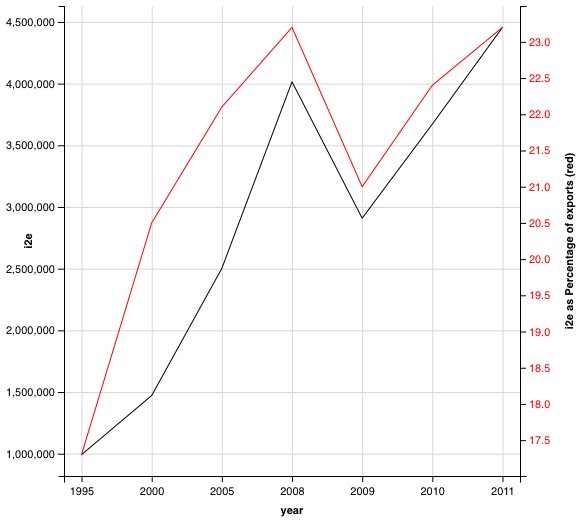
\includegraphics[scale=0.4]{i2epercentage.png}
\caption{The development of GVC integration over time}
\end{figure}

Looking at sectoral $fvax$ averages, Figure \ref{fig:i2e_s} reveals that the sectors exhibiting the highest dependency on foreign inputs are heavy manufactures such as motor vehicles (MTR), other transport equipment (TRQ) and the metal industry (MET) as well as computers and electronics (CEQ and ELQ). In particular, the transport equipment and electronics industry are strongly engaged in GVCs having highly international production networks. For instance, Apple's iPhone contains inputs from 9 to 10 countries while the Boeing 787 production spans more than 5 countries. These sectors are typically close to final demand or depend on imported raw materials.

The bottom 6 industries are primary and services sectors such as agriculture (AGR), mining (MIN), R\&D and business services (BZS), or wholesale and retail trade (WRT). These sectors are typically located upstream in the supply chain far from final demand and have high high value added to output ratios.

Naturally then, things are reversed when we look at the corresponding forward linkage GVC measure, $dvar$. It captures the amount of domestic value added in foreign exports and thus quantifies how important domestic industries are for foreign export production. Here, Figure \ref{fig:e2r_s} depicts that this indicator is dominated by the same upstream industries that are at the bottom of the $fvax$ ranking such as mining or financial and telecommunication services (FIN and PTL). This shows that these industries are also strongly engaged in GVCs but their participation is of a different type. They primarily supply important inputs but do not serve final demand. 

With respect to services, it is also indicative of the servicification of manufacturing as described by \citet{ribaetal15}. This means that an increasing share of manufacturing gross exports is actually value added generated in services sectors and then embedded in the intermediate exports of manufacturers. This importance of services sectors for exports cannot be seen from standard gross trade statistics and thus constitutes a major advantage of trade in value added measures. It is also indicative of a growing internationalisation of services. Increasingly, services are being offshored and sourced from abroad. In that respect, it is also interesting to note that despite the low absolute $fvax$ shares, it is in services where a lot of the growth in $fvax$ has taken place. As can be seen in Figure \ref{fig:i2e_st}, five out of the six sectors with the highest growth in $fvax$ shares are services sectors.

\section{New trends and patterns in GVCs}\label{sec:news}



\section{Conclusion}\label{sec:conclusion}

\clearpage

\bibliographystyle{chicago}
\bibliography{GVCandLMICs}

\clearpage

\end{document}
